\documentclass[a4paper]{article}
\usepackage[utf8]{vietnam}
%\usepackage[utf8]{inputenc} %dành cho english
\usepackage{amsmath} %packet math
%
\usepackage{hyperref}
\hypersetup{colorlinks=true,linkcolor=blue,urlcolor=blue,citecolor=blue} % hiển thị màu đánh dấu (1)  (2) hoặc đường link ,...
\usepackage{graphicx} %Thư viện vẽ bảng

\title{Hello World!}

\author{Your Name}

\date{\today}

\begin{document}
\maketitle
\begin{abstract}
Các bạn đọc có cách viết gọn hơn, trình bày đẹp hơn,... có thể liên hệ và trao đổi với để mọi người học hỏi thêm \\
Tài liệu mà mình tham khảo trên mạng: cái link đầu là bài viết này, link sau là tham khảo (khá chi tiết).\\ 
\url{https://guides.nyu.edu/c.php?g=601858&p=4168140}\\
\url{https://blogchiasekienthuc.com/series/huong-dan-su-dung-latex}\\

\end{abstract}

\section{Getting Stared}
\textbf{Hello World!} Today I am learing \LaTeX. \LaTeX is a great program for writing math. I can write in line math such as $a^2 + b^2 = c^2$. I can also give equations their own space:
$\gamma^2+\theta^2=\omega^2$
\[\gamma^2+\theta^2=\omega^2\]
\begin{equation}
\gamma^2+\theta^2=\omega^2\
\end{equation}
"Maxwell's equations" are named for James Clark Maxwell and are as follow:
% & để căn chỉnh, nếu muốn căn chỉnh lần hai thì &&
% \frac{num}{den} in ra phân số num/den
\begin{align}
\vec{\nabla} \cdot \vec{E} \quad &= \quad\frac{\rho}{\epsilon} &&\text{Gauss's Law}\label{eq:GL}\\
\vec{\nabla} \cdot \vec{B} \quad &= \quad 0 &&\text{Gauss's Law for Mahnetism}\label{2}\\
\vec{\nabla} \times \vec{E} \quad &= \hspace{10pt}-\frac{\partial{\vec{B}}}{\partial{t}}
\vec{\nabla} &&\text{Faraday's Law of Induction}\label{3}\\
\vec{\nabla} \times \vec{B} \quad &= \quad \mu_{0}\left(\epsilon\frac{\partial{\vec{E}}}{partial{t}}+\vec{J}\right) &&text{Ampere's Circuital Law}\label{4}
\end{align}
Equations \ref{eq:GL}, \ref{2}, \ref{3}, and \ref{4} are some of most important in Physics.

%equation: phương trình, align căn chỉnh
%equation*: không có đánh số

\section{What about Matrix Equation?} 
\begin{equation*}
\begin{pmatrix}
a_{11} & a_{12} & \dots & a_{1n}\\
a_{21} & a_{22} & \dots & a_{2n}\\
\vdots & \vdots & \ddots & \vdots\\
a_{n1} & a_{n2}& \dots & a_{nn}
\end{pmatrix}
\begin{bmatrix}
v_(1)\\
v_(2)\\
\vdots\\
v_(n)\\
\end{bmatrix}
=
\begin{matrix}
w_{1}\\ w_{2}\\ \vdots \\ w_{n}
\end{matrix}
\end{equation*}

\section{Table and Figures} %3
Creating a Table is not unlike creating a matrix:\\
\begin{table}[h]
\centering
\caption{This is a table that shows how to create different lines as well as different justification}
\begin{tabular}{|l||c|c|r|}
\hline  
$x$&1&2&3\\
\hline
$f(x)$&4&8&12\\
f(x)&4&8&12\\
\hline
\end{tabular}
\end{table}

 
\section{Insert Picture} %4
How to insert picture in \LaTeX \\
Use Wizards $->$ Insert Garphic
\begin{figure}[tph]
\centering
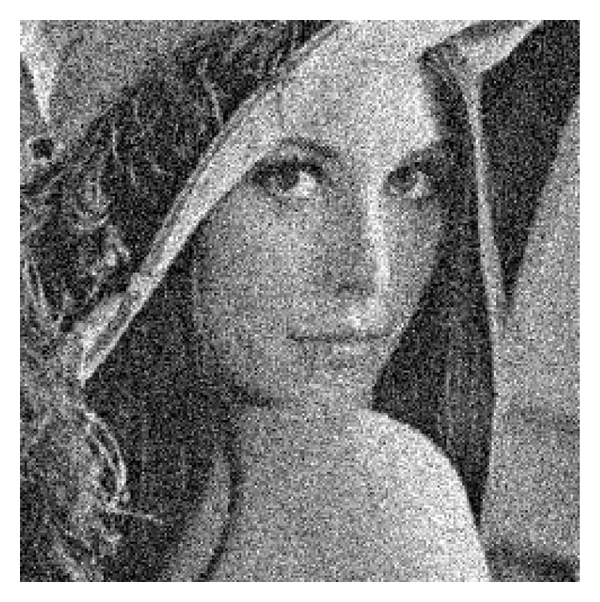
\includegraphics[width=0.7\linewidth]{lena}
\caption{This is Lena}
\end{figure}

\section{Bibliography} %Phần thư mục
You will probably want references in your document so that you can cite articles like \cite{gratzer2007more}\\
Bibliography.bib là thư mục tự tạo chứa phần reference\\
Tìm Bib TeX trên Google Scholar\\
Ảnh minh hoạt hướng dẫn:\\

\begin{figure}[!ht]
\begin{minipage}[b]{0.4\textwidth}
\centering
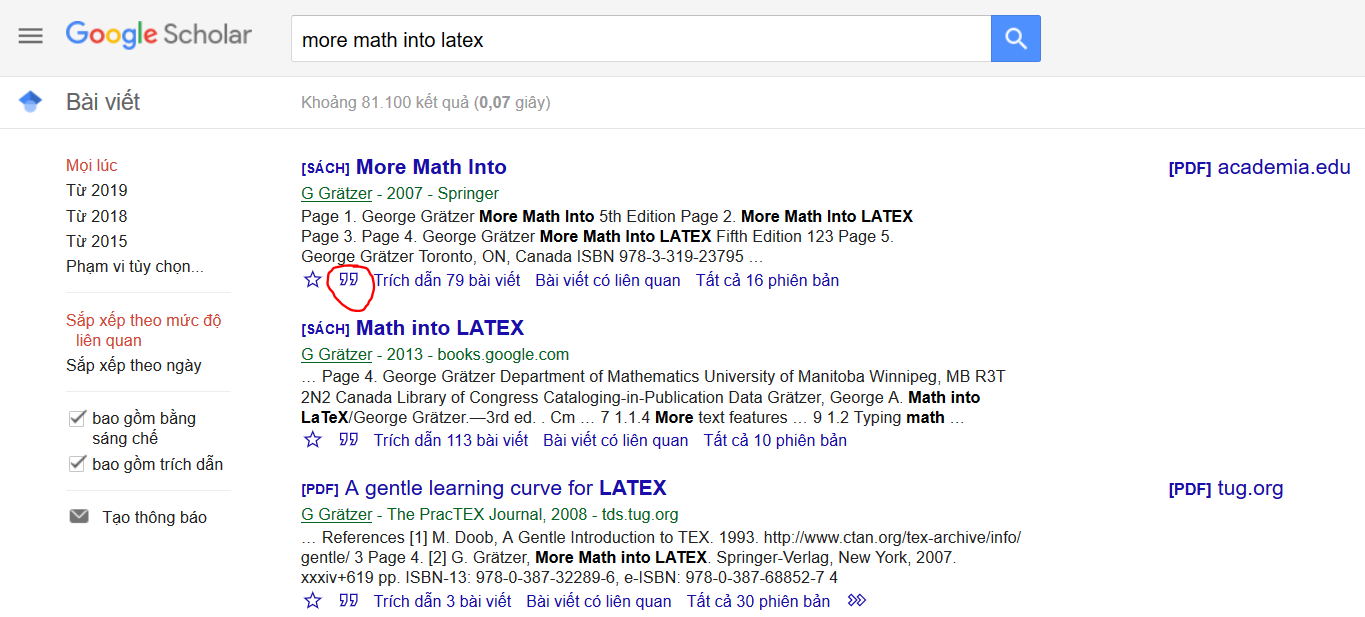
\includegraphics[height=8cm,width=12cm]{huongdan1}
\caption{Bước 1}\label{fig:*1}
\end{minipage}

\begin{minipage}[t]{0.4\textwidth}
\centering
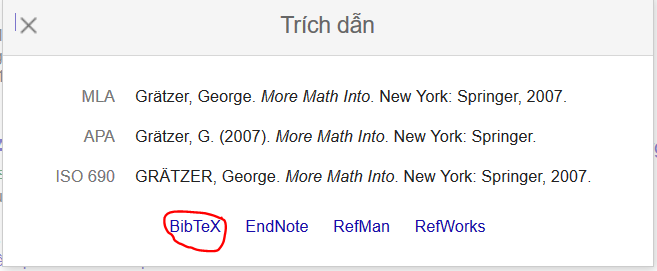
\includegraphics[height=8cm,width=12cm]{huongdan2}
\caption{Bước 2}\label{fig:*2}
\end{minipage}
\end{figure}


\bibliographystyle{plain}
\bibliography{Bibligra} %Chỉ để Bibligra, KHÔNG ĐỂ Bibligra.bib

\end{document}

